\subsection{Controller}

\begin{figure}[h]
	\centering
	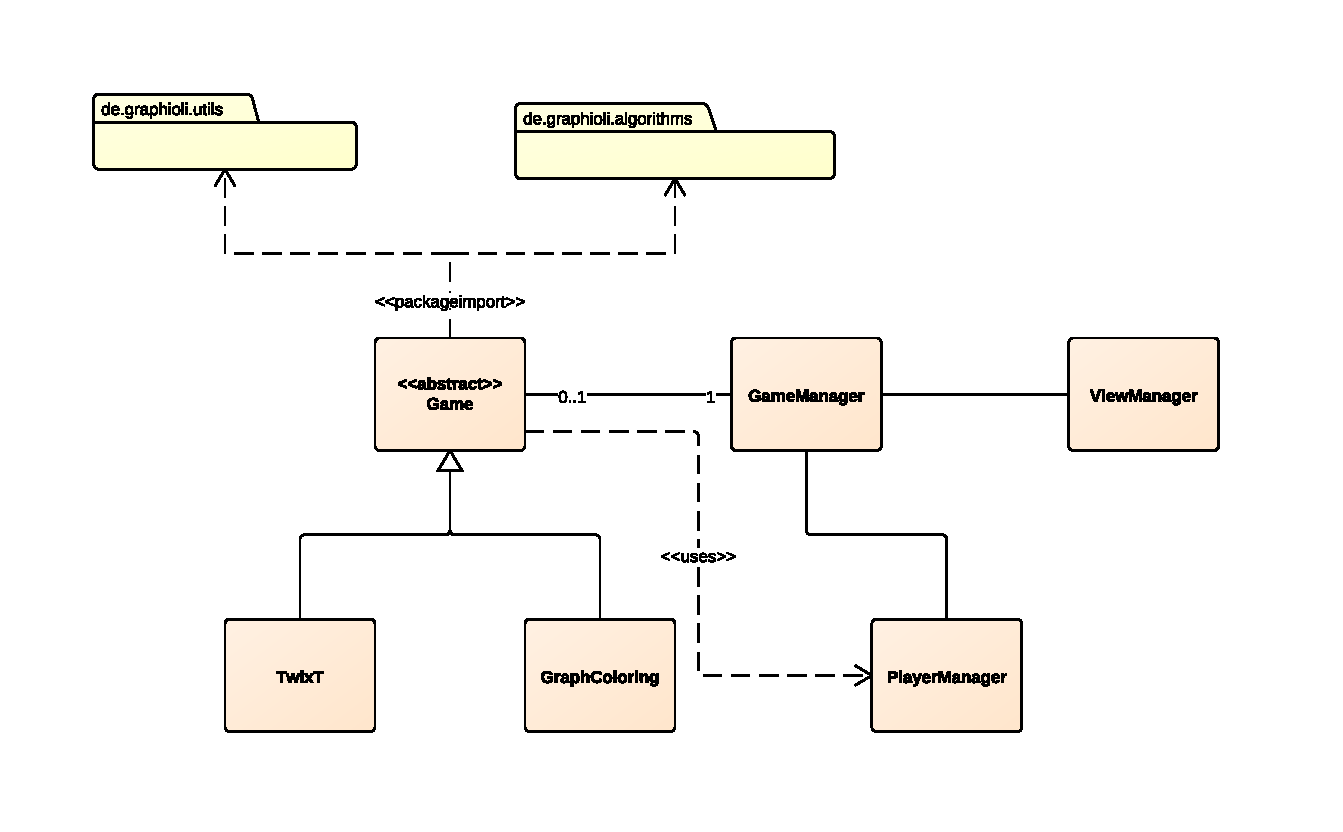
\includegraphics[page=1,width=\textwidth,keepaspectratio]{controllerClassDiagram.pdf}
	\caption{Controller class diagram.}
	\label{img:controllerClassDiagram}
\end{figure}

\pagebreak

% Game
\abstractclass{Game}{game}
This is the class that every \gls{game} has to inherit from, when using the \graphioli framework. It defines the callback functions that the game developer needs in order to implement the game's logic. \\

\subclasses{cls:graphcoloring, cls:twixt}

\centerdash

\paragraph*{Method Summary}
\paragraph*{}
\begin{longtable}{Lp{10cm}}
	\startmethodtable
	\method{public final boolean}{registerController(GameManager manager)}{game:registercontroller} \\
	& Associates this \texttt{Game} with a \ref{cls:gamemanager}. \\
	\method{protected final GameManager}{getGameManager()}{game:getgamemanager} \\
	& Returns the associated \ref{cls:gamemanager}. \\
	\method{protected abstract boolean}{onVertexClick(VisualVertex vertex)}{game:onvertexclick} \\
	& Called when a player clicks on a \ref{cls:visualvertex}. \\
	\method{protected abstract boolean}{onEmptyGridPointClick(GridPoint gridPoint)}{game:onemptygridpointclick} \\
	& Called when a player clicks on a \ref{cls:gridpoint} that has no \ref{cls:visualvertex} on it. \\
	\method{protected abstract boolean}{onGameInit()}{game:ongameinit} \\
	& Called after a \texttt{Game} has been instantiated. \\
	\method{protected abstract boolean}{onGameStart()}{game:ongamestart} \\
	& Called immediately before a \texttt{Game} gets (re)started. \\
	\method{protected boolean}{onKeyRelease(int keyCode)}{game:onkeyrelease} \\
	& Called when a player releases a keyboard key.\\
	\method{protected boolean}{onMenuItemClick(MenuItem item)}{game:onmenuitemclick} \\
	& Called when a player clicks on a custom \texttt{MenuItem}. \\
	\hline
\end{longtable}

\pagebreak

% GameManager
\class{GameManager}{gamemanager}
This is the framework's central class, connecting the actual game with the \texttt{model} and the \texttt{view}. Any communication between \texttt{model}, \texttt{view} and \texttt{controller} will be managed by the \texttt{GameManager}. \\

\centerdash

\paragraph*{Method Summary}
\paragraph*{}
\begin{longtable}{Lp{10cm}}
	\startmethodtable
	\method{public static void}{main(String[ ] args)}{gm:main} \\
	& The main method initializes the \texttt{GameManager} to start the whole application. \\
	\method{private boolean}{openGameExplorer()}{gm:opengameexplorer} \\
	& Starts the \ref{cls:gameexplorer}. \\
	\method{private boolean}{killGame()}{gm:killgame} \\
	& Kills the currently running game. \\
	\method{public boolean}{startGame(GameDefinition gameDefinition)}{gamemanager:startgame} \\
	& Starts the game specified by the \ref{cls:gamedefinition}. \\
	\method{public boolean}{loadGame(File savegame)}{gm:loadgame} \\
	& Creates a \ref{cls:gamecapsule} from the savegame file and loads the information to start the game in the saved state. \\
	\method{public boolean}{saveGame(File savegame)}{gm:savegame} \\
	& Creates a \ref{cls:gamecapsule} and serializes it into a savegame file to save the current state of the game. \\
	\method{public boolean}{finishGame()}{gm:finishgame} \\
	& Finishes the game and displays a default pop-up for single player games. \\
	\method{public boolean}{finishGame(Player winner)}{gm:finishgameWinner} \\
	& Finishes the game and displays the winning \ref{cls:player} in a pop-up.  \\
	\method{public boolean}{restartGame()}{gm:restartgame} \\
	& Restarts the game and resets the \ref{cls:gameboard} and \ref{cls:player}s. \\
	\method{public boolean}{closeGame()}{gm:closegame} \\
	& Closes the game with its \ref{cls:gamewindow} and returns the focus to the \ref{cls:gameexplorer}. \\
	\method{public PlayerManager}{getPlayerManager()}{gm:getplayermanager} \\
	& Returns the \ref{cls:playermanager} associated with this \texttt{GameManager}.\\
	\method{public ViewManager}{getViewManager()}{gm:getviewmanager} \\
	& Returns the \ref{cls:viewmanager} associated with this \texttt{GameManager}.\\
	\method{public GameBoard}{getGameBoard()}{gm:getgameboard} \\
	& Returns the \ref{cls:gameboard} associated with this \texttt{GameManager}.\\
	\hline
\end{longtable}

\pagebreak

% ViewManager
\class{ViewManager}{viewmanager}
This class acts as an interface between the \gls{GUI} and the other parts of the \gls{framework}. It pushes update notifications to the view and receives user input from it. \\

\centerdash

\paragraph*{Method Summary}
\paragraph*{}
\begin{longtable}{Lp{10cm}}
	\startmethodtable
	\method{public}{ViewManager(GameManager gameManager)}{viewmanager:viewmanager} \\
	& Creates a new \texttt{ViewManager} associated with the given \ref{cls:gamemanager}. \\
	\method{public boolean}{updatePlayerStatus(Player player)}{viewmanager:updateplayerstatus} \\
	& Notifies the \ref{cls:view} to display the given \ref{cls:player} as active. \\
	\method{public boolean}{onGridPointClick(GridPoint gridpoint)}{viewmanager:ongridpointclick} \\
	& Callback function used by the \ref{cls:view} to notify about a click on a \ref{cls:gridpoint}.  \\
	\method{public boolean}{onKeyRelease(int keycode)}{viewmanager:onkeyrelease} \\
	& Callback function used by the \ref{cls:view} to notify about a key release. \\
	\method{public boolean}{displayErrorMessage(String message)}{viewmanager:displayerrormessage} \\
	& Notifies the \ref{cls:view} to display the error message. \\
	\method{public boolean}{displayPopUp(String message)}{viewmanager:displaypopup} \\
	& Notifies the \ref{cls:view} to display the given message in a pop-up. \\
	\method{public boolean}{addGameMenuItem(MenuItem item}{viewmanager:addgamemenuitem} \\
	& Notifies the \ref{cls:view} to add the given \texttt{MenuItem} to the menu. \\
	\method{public boolean}{onMenuItemClick(MenuItem item)}{viewmanager:onmenuitemclick} \\
	& Callback function used by the \ref{cls:view} to notify about a click on a previously added \texttt{MenuItem}.  \\
	\method{public GameManager}{getGameManager()}{viewmanager:getgamemanager} \\
	& Returns the associated \ref{cls:gamemanager}. \\
	\method{public boolean}{setVisualVertexSet(int size)}{viewmanager:setvisualvertexsize} \\
	& Notifies the \ref{cls:view} to change the \texttt{size} of the \texttt{VisualVertices} to the given value. \\
	\hline
\end{longtable}

\pagebreak

% PlayerManager
\class{PlayerManager}{playermanager}
This class is responsible for keeping information about a game's \ref{cls:player}s.  \\

\centerdash

\paragraph*{Method Summary}
\paragraph*{}
\begin{longtable}{Lp{10cm}}
	\startmethodtable
	\method{public}{PlayerManager(Iterable<Player> players)}{pm:playermanager} \\
	& Constructs a \texttt{PlayerManager} with the given set of \ref{cls:player}s. \\
	\method{private boolean}{initializePlayers()}{pm:initializeplayers} \\
	& Initializes registered \ref{cls:player}s. \\
	\method{public Iterable<Player>}{getPlayers()}{pm:getplayers} \\
	& Returns the list of \ref{cls:player}s managed by this instance. \\
	\method{public Player}{getActivePlayer()}{pm:getactiveplayer} \\
	& Returns the \ref{cls:player}, who is currently active. \\
	\method{public Player}{nextPlayer()}{pm:nextplayer} \\
	& Sets the next \ref{cls:player} in the list to active. \\
	\hline
\end{longtable}

\pagebreak

\subsubsection{Games}

%GraphColoring
\class{GraphColoring}{graphcoloring}
\createindentedlist{de.graphioli.controller.Game, de.graphioli.controller.GraphColoring}
Our implemented game containing the game's logic of \graphcoloring in single and multiplayer mode. \\

\centerdash

\paragraph*{Method Summary}
\paragraph*{}
\begin{longtable}{Lp{10cm}}
	\startmethodtable
	\method{private boolean}{generateBoard()}{gc:generateboard} \\
	& Generates the \ref{cls:gameboard} used to play the game. \\
	\method{protected abstract boolean}{onVertexClick(VisualVertex vertex)}{gc:onvertexclick} \\
	& Colors the given \ref{cls:vertex} -- if possible -- and decides if the game is finished by this move. \\
	\method{protected abstract boolean}{onEmptyGridPointClick(GridPoint gridPoint)}{gc:onemptygridpointclick} \\
	& Has no function in this game. \\
	\method{protected abstract boolean}{onGameInit()}{gc:ongameinit} \\
	& Decides whether the game is started in \texttt{single} or \texttt{multiplayer mode}. \\
	\method{protected abstract boolean}{onGameStart()}{gc:ongamestart} \\
	& (Re)builds the \ref{cls:gameboard} using \ref{gc:generateboard}. \\
	\hline
\end{longtable}

\pagebreak

%TwixT
\class{TwixT}{twixt}
\createindentedlist{de.graphioli.controller.Game, de.graphioli.controller.TwixT}
Our implemented game containing the game's logic of \twixt. \\

\centerdash

\paragraph*{Method Summary}
\paragraph*{}
\begin{longtable}{Lp{10cm}}
	\startmethodtable
	\method{private boolean}{generateBoard()}{twixt:generateboard} \\
	& Generates the \ref{cls:gameboard} used to play the game. \\
	\method{protected abstract boolean}{onVertexClick(VisualVertex vertex)}{twixt:onvertexclick} \\
	& Selects a tower on the \ref{cls:gameboard} and creates an \ref{cls:edge} between this \ref{cls:vertex} and the one previously selected if they belong to the same \ref{cls:player} and the new \ref{cls:edge} would not intersect with another one.
	It then checks if the baselines are connected and the game is finished.\\
	\method{protected abstract boolean}{onEmptyGridPointClick(GridPoint gridPoint)}{twixt:onemptygridpointclick} \\
	& Sets a new \ref{cls:twixtvertex} belonging to the active \ref{cls:player} onto the given \ref{cls:gridpoint}, if possible. \\
	\method{protected abstract boolean}{onGameInit()}{twixt:ongameinit} \\
	& Initilaizes the \ref{cls:twixtvertex} class. \\
	\method{protected abstract boolean}{onGameStart()}{twixt:ongamestart} \\
	& (Re)builds the \ref{cls:gameboard} using \ref{twixt:generateboard}. \\	
	\hline
\end{longtable}